\chapter{Amortizirana analiza}

\index{amortizirana analiza}

Vremensku složenost algoritma
često je jednostavno analizirati
samo pregledavanjem strukture
algoritma:
koje petlje algoritam sadrži
i koliko se puta te petlje izvode.
Ipak, ponekad izravna analiza
ne daje pravu sliku o efikasnosti algoritma.

\key{Amortizirana analiza} može se koristiti za analizu
algoritama koji sadrže operacije čija
vremenska složenost varira.
Ideja je procijeniti ukupno vrijeme potrošeno na
sve takve operacije tijekom
izvođenja algoritma, umjesto da se usredotočimo
na pojedinačne operacije.

\section{Metoda dvaju pokazivača}

\index{metoda dvaju pokazivača}

U \key{metodi dvaju pokazivača}
koriste se dva pokazivača za
prolaz kroz vrijednosti niza.
Oba pokazivača mogu se kretati samo u jednom smjeru,
što osigurava da algoritam radi efikasno.
Zatim razmatramo dva zadatka koja se mogu riješiti
metodom dvaju pokazivača.

\subsubsection{Suma podniza}

Kao prvi primjer,
razmotrimo zadatak u kojem je
dan niz od $n$ pozitivnih cijelih brojeva
i ciljana suma $x$,
a želimo naći podniz čija je suma $x$
ili javiti da takav podniz ne postoji.

Na primjer, niz
\begin{center}
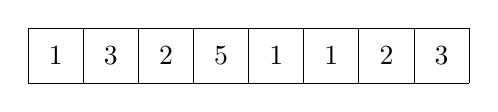
\begin{tikzpicture}[scale=0.7]
\draw (0,0) grid (8,1);

\node at (0.5,0.5) {$1$};
\node at (1.5,0.5) {$3$};
\node at (2.5,0.5) {$2$};
\node at (3.5,0.5) {$5$};
\node at (4.5,0.5) {$1$};
\node at (5.5,0.5) {$1$};
\node at (6.5,0.5) {$2$};
\node at (7.5,0.5) {$3$};
\end{tikzpicture}
\end{center}
sadrži podniz čija je suma 8:
\begin{center}
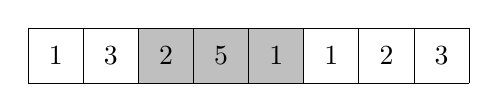
\begin{tikzpicture}[scale=0.7]
\fill[color=lightgray] (2,0) rectangle (5,1);
\draw (0,0) grid (8,1);

\node at (0.5,0.5) {$1$};
\node at (1.5,0.5) {$3$};
\node at (2.5,0.5) {$2$};
\node at (3.5,0.5) {$5$};
\node at (4.5,0.5) {$1$};
\node at (5.5,0.5) {$1$};
\node at (6.5,0.5) {$2$};
\node at (7.5,0.5) {$3$};
\end{tikzpicture}
\end{center}

Ovaj zadatak može se riješiti u
$O(n)$ vremenu koristeći metodu dvaju pokazivača.
Ideja je održavati pokazivače koji pokazuju na
prvu i posljednju vrijednost podniza.
U svakom koraku lijevi pokazivač pomiče se jedan korak
udesno, a desni pokazivač pomiče se udesno
sve dok je suma nastalog podniza najviše $x$.
Ako suma postane točno $x$,
rješenje je nađeno.

Kao primjer, razmotrimo sljedeći niz
i ciljanu sumu $x=8$:
\begin{center}
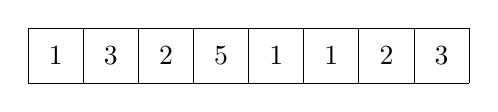
\begin{tikzpicture}[scale=0.7]
\draw (0,0) grid (8,1);

\node at (0.5,0.5) {$1$};
\node at (1.5,0.5) {$3$};
\node at (2.5,0.5) {$2$};
\node at (3.5,0.5) {$5$};
\node at (4.5,0.5) {$1$};
\node at (5.5,0.5) {$1$};
\node at (6.5,0.5) {$2$};
\node at (7.5,0.5) {$3$};
\end{tikzpicture}
\end{center}

Početni podniz sadrži vrijednosti
1, 3 i 2 čija je suma 6:

\begin{center}
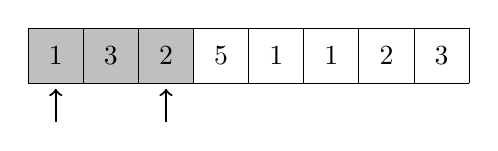
\begin{tikzpicture}[scale=0.7]
\fill[color=lightgray] (0,0) rectangle (3,1);
\draw (0,0) grid (8,1);

\node at (0.5,0.5) {$1$};
\node at (1.5,0.5) {$3$};
\node at (2.5,0.5) {$2$};
\node at (3.5,0.5) {$5$};
\node at (4.5,0.5) {$1$};
\node at (5.5,0.5) {$1$};
\node at (6.5,0.5) {$2$};
\node at (7.5,0.5) {$3$};

\draw[thick,->] (0.5,-0.7) -- (0.5,-0.1);
\draw[thick,->] (2.5,-0.7) -- (2.5,-0.1);
\end{tikzpicture}
\end{center}

Zatim se lijevi pokazivač pomiče jedan korak udesno.
Desni pokazivač se ne pomiče, jer bi inače
suma podniza premašila $x$.

\begin{center}
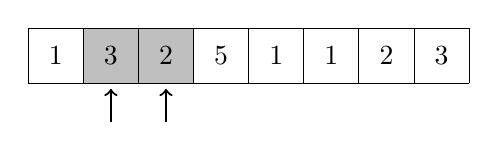
\begin{tikzpicture}[scale=0.7]
\fill[color=lightgray] (1,0) rectangle (3,1);
\draw (0,0) grid (8,1);

\node at (0.5,0.5) {$1$};
\node at (1.5,0.5) {$3$};
\node at (2.5,0.5) {$2$};
\node at (3.5,0.5) {$5$};
\node at (4.5,0.5) {$1$};
\node at (5.5,0.5) {$1$};
\node at (6.5,0.5) {$2$};
\node at (7.5,0.5) {$3$};

\draw[thick,->] (1.5,-0.7) -- (1.5,-0.1);
\draw[thick,->] (2.5,-0.7) -- (2.5,-0.1);
\end{tikzpicture}
\end{center}

Ponovno se lijevi pokazivač pomiče jedan korak udesno,
a ovaj put desni pokazivač pomiče se tri
koraka udesno.
Suma podniza je $2+5+1=8$, pa je nađen podniz
čija je suma $x$.

\begin{center}
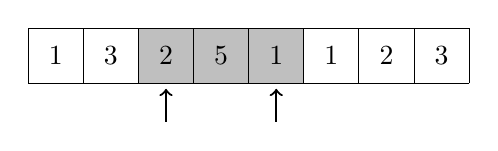
\begin{tikzpicture}[scale=0.7]
\fill[color=lightgray] (2,0) rectangle (5,1);
\draw (0,0) grid (8,1);

\node at (0.5,0.5) {$1$};
\node at (1.5,0.5) {$3$};
\node at (2.5,0.5) {$2$};
\node at (3.5,0.5) {$5$};
\node at (4.5,0.5) {$1$};
\node at (5.5,0.5) {$1$};
\node at (6.5,0.5) {$2$};
\node at (7.5,0.5) {$3$};

\draw[thick,->] (2.5,-0.7) -- (2.5,-0.1);
\draw[thick,->] (4.5,-0.7) -- (4.5,-0.1);
\end{tikzpicture}
\end{center}

Vrijeme izvođenja algoritma ovisi o
broju koraka koje napravi desni pokazivač.
Iako ne postoji korisna gornja ograda na to koliko koraka
pokazivač može napraviti u \emph{jednom} koraku petlje,
znamo da se pokazivač pomakne \emph{ukupno}
$O(n)$ koraka tijekom algoritma,
jer se pomiče samo udesno.

Budući da se i lijevi i desni pokazivač
pomiču $O(n)$ koraka tijekom algoritma,
algoritam radi u $O(n)$ vremenu.

\subsubsection{Zadatak 2SUM}

\index{zadatak 2SUM}

Drugi zadatak koji se može riješiti
metodom dvaju pokazivača je sljedeći zadatak,
poznat i kao \key{zadatak 2SUM}:
dan je niz od $n$ brojeva i
ciljana suma $x$; treba naći
dvije vrijednosti niza takve da je njihova suma $x$,
ili javiti da takve vrijednosti ne postoje.

Da bismo riješili zadatak, najprije
sortiramo vrijednosti niza u rastućem redoslijedu.
Nakon toga prolazimo kroz niz koristeći
dva pokazivača.
Lijevi pokazivač počinje na prvoj vrijednosti
i u svakom koraku pomiče se jedan korak udesno.
Desni pokazivač počinje na posljednjoj vrijednosti
i uvijek se pomiče ulijevo dok suma
lijeve i desne vrijednosti ne postane najviše $x$.
Ako je suma točno $x$,
rješenje je nađeno.

Na primjer, razmotrimo sljedeći niz
i ciljanu sumu $x=12$:
\begin{center}
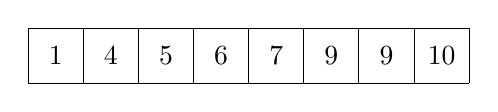
\begin{tikzpicture}[scale=0.7]
\draw (0,0) grid (8,1);

\node at (0.5,0.5) {$1$};
\node at (1.5,0.5) {$4$};
\node at (2.5,0.5) {$5$};
\node at (3.5,0.5) {$6$};
\node at (4.5,0.5) {$7$};
\node at (5.5,0.5) {$9$};
\node at (6.5,0.5) {$9$};
\node at (7.5,0.5) {$10$};
\end{tikzpicture}
\end{center}

Početni položaji pokazivača
su sljedeći.
Suma vrijednosti je $1+10=11$
što je manje od $x$.

\begin{center}
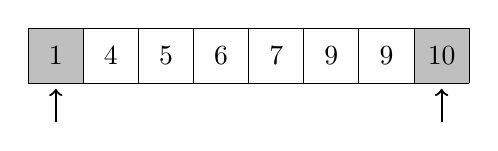
\begin{tikzpicture}[scale=0.7]
\fill[color=lightgray] (0,0) rectangle (1,1);
\fill[color=lightgray] (7,0) rectangle (8,1);
\draw (0,0) grid (8,1);

\node at (0.5,0.5) {$1$};
\node at (1.5,0.5) {$4$};
\node at (2.5,0.5) {$5$};
\node at (3.5,0.5) {$6$};
\node at (4.5,0.5) {$7$};
\node at (5.5,0.5) {$9$};
\node at (6.5,0.5) {$9$};
\node at (7.5,0.5) {$10$};

\draw[thick,->] (0.5,-0.7) -- (0.5,-0.1);
\draw[thick,->] (7.5,-0.7) -- (7.5,-0.1);
\end{tikzpicture}
\end{center}

Zatim se lijevi pokazivač pomiče jedan korak udesno.
Desni pokazivač pomiče se tri koraka ulijevo,
i suma postaje $4+7=11$.

\begin{center}
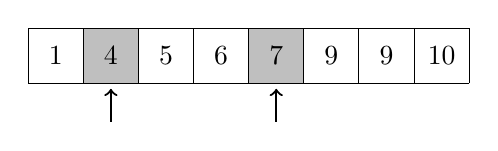
\begin{tikzpicture}[scale=0.7]
\fill[color=lightgray] (1,0) rectangle (2,1);
\fill[color=lightgray] (4,0) rectangle (5,1);
\draw (0,0) grid (8,1);

\node at (0.5,0.5) {$1$};
\node at (1.5,0.5) {$4$};
\node at (2.5,0.5) {$5$};
\node at (3.5,0.5) {$6$};
\node at (4.5,0.5) {$7$};
\node at (5.5,0.5) {$9$};
\node at (6.5,0.5) {$9$};
\node at (7.5,0.5) {$10$};

\draw[thick,->] (1.5,-0.7) -- (1.5,-0.1);
\draw[thick,->] (4.5,-0.7) -- (4.5,-0.1);
\end{tikzpicture}
\end{center}

Nakon toga lijevi pokazivač ponovno se pomiče jedan korak udesno.
Desni pokazivač se ne pomiče, a nađeno je rješenje
$5+7=12$.

\begin{center}
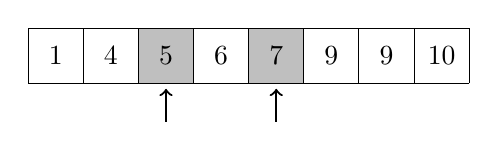
\begin{tikzpicture}[scale=0.7]
\fill[color=lightgray] (2,0) rectangle (3,1);
\fill[color=lightgray] (4,0) rectangle (5,1);
\draw (0,0) grid (8,1);

\node at (0.5,0.5) {$1$};
\node at (1.5,0.5) {$4$};
\node at (2.5,0.5) {$5$};
\node at (3.5,0.5) {$6$};
\node at (4.5,0.5) {$7$};
\node at (5.5,0.5) {$9$};
\node at (6.5,0.5) {$9$};
\node at (7.5,0.5) {$10$};

\draw[thick,->] (2.5,-0.7) -- (2.5,-0.1);
\draw[thick,->] (4.5,-0.7) -- (4.5,-0.1);
\end{tikzpicture}
\end{center}

Vrijeme izvođenja algoritma je
$O(n \log n)$, jer najprije sortira
niz u $O(n \log n)$ vremenu,
a zatim se oba pokazivača pomiču $O(n)$ koraka.

Napomenimo da je zadatak moguće riješiti
i na drugi način u $O(n \log n)$ vremenu koristeći binarno traženje.
U takvom rješenju prolazimo kroz niz
i za svaku vrijednost niza pokušavamo naći drugu
vrijednost koja daje sumu $x$.
To se može učiniti izvođenjem $n$ binarnih traženja,
od kojih svako traje $O(\log n)$ vremena.

\index{zadatak 3SUM}
Teži zadatak je 
\key{zadatak 3SUM} koji traži
da se nađu \emph{tri} vrijednosti niza
čija je suma $x$.
Koristeći ideju gornjeg algoritma,
ovaj zadatak može se riješiti u $O(n^2)$ vremenu\footnote{Dugo se
mislilo da rješavanje
zadatka 3SUM efikasnije od $O(n^2)$ vremena
nije moguće.
Međutim, 2014. godine pokazalo se \cite{gro14}
da to nije slučaj.}.
Vidite li kako?

\section{Najbliži manji elementi}

\index{najbliži manji elementi}

Amortizirana analiza često se koristi za
procjenu broja operacija
izvedenih nad strukturom podataka.
Operacije mogu biti neravnomjerno raspoređene tako
da se većina operacija dogodi tijekom
određene faze algoritma, ali je ukupan
broj operacija ograničen.

Kao primjer, razmotrimo zadatak
nalaženja, za svaki element niza,
\key{najbližeg manjeg elementa}, tj.
prvog manjeg elementa koji u nizu
prethodi tom elementu.
Moguće je da takav element ne postoji,
u kojem slučaju algoritam to treba javiti.
Zatim ćemo vidjeti kako se zadatak može
efikasno riješiti pomoću strukture stoga.

Prolazimo kroz niz slijeva nadesno
i održavamo stog elemenata niza.
Na svakom položaju u nizu uklanjamo elemente sa stoga
dok element na vrhu ne postane manji od
trenutnog elementa ili dok stog ne ostane prazan.
Zatim javljamo da je element na vrhu
najbliži manji element trenutnog elementa,
ili, ako je stog prazan, da takav element ne postoji.
Na kraju dodajemo trenutni element na stog.

Kao primjer, razmotrimo sljedeći niz:
\begin{center}
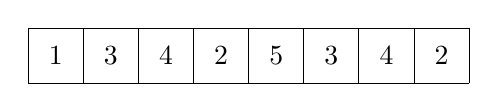
\begin{tikzpicture}[scale=0.7]
\draw (0,0) grid (8,1);

\node at (0.5,0.5) {$1$};
\node at (1.5,0.5) {$3$};
\node at (2.5,0.5) {$4$};
\node at (3.5,0.5) {$2$};
\node at (4.5,0.5) {$5$};
\node at (5.5,0.5) {$3$};
\node at (6.5,0.5) {$4$};
\node at (7.5,0.5) {$2$};
\end{tikzpicture}
\end{center}

Najprije se elementi 1, 3 i 4 dodaju na stog,
jer je svaki element veći od prethodnog elementa.
Dakle, najbliži manji element broja 4 je 3,
a najbliži manji element broja 3 je 1.
\begin{center}
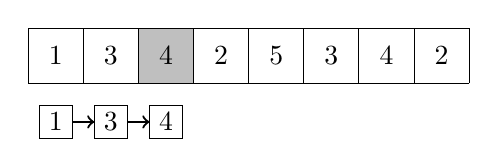
\begin{tikzpicture}[scale=0.7]
\fill[color=lightgray] (2,0) rectangle (3,1);
\draw (0,0) grid (8,1);

\node at (0.5,0.5) {$1$};
\node at (1.5,0.5) {$3$};
\node at (2.5,0.5) {$4$};
\node at (3.5,0.5) {$2$};
\node at (4.5,0.5) {$5$};
\node at (5.5,0.5) {$3$};
\node at (6.5,0.5) {$4$};
\node at (7.5,0.5) {$2$};

\draw (0.2,0.2-1.2) rectangle (0.8,0.8-1.2);
\draw (1.2,0.2-1.2) rectangle (1.8,0.8-1.2);
\draw (2.2,0.2-1.2) rectangle (2.8,0.8-1.2);

\node at (0.5,0.5-1.2) {$1$};
\node at (1.5,0.5-1.2) {$3$};
\node at (2.5,0.5-1.2) {$4$};

\draw[->,thick] (0.8,0.5-1.2) -- (1.2,0.5-1.2);
\draw[->,thick] (1.8,0.5-1.2) -- (2.2,0.5-1.2);
\end{tikzpicture}
\end{center}

Sljedeći element 2 manji je od dva gornja
elementa na stogu.
Dakle, elementi 3 i 4 uklanjaju se sa stoga,
a zatim se element 2 dodaje na stog.
Njegov najbliži manji element je 1:
\begin{center}
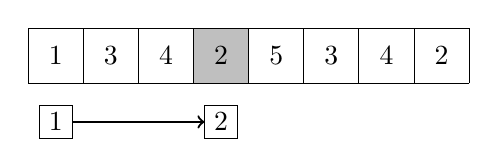
\begin{tikzpicture}[scale=0.7]
\fill[color=lightgray] (3,0) rectangle (4,1);
\draw (0,0) grid (8,1);

\node at (0.5,0.5) {$1$};
\node at (1.5,0.5) {$3$};
\node at (2.5,0.5) {$4$};
\node at (3.5,0.5) {$2$};
\node at (4.5,0.5) {$5$};
\node at (5.5,0.5) {$3$};
\node at (6.5,0.5) {$4$};
\node at (7.5,0.5) {$2$};

\draw (0.2,0.2-1.2) rectangle (0.8,0.8-1.2);
\draw (3.2,0.2-1.2) rectangle (3.8,0.8-1.2);

\node at (0.5,0.5-1.2) {$1$};
\node at (3.5,0.5-1.2) {$2$};

\draw[->,thick] (0.8,0.5-1.2) -- (3.2,0.5-1.2);
\end{tikzpicture}
\end{center}

Zatim je element 5 veći od elementa 2,
pa će biti dodan na stog, a
njegov najbliži manji element je 2:
\begin{center}
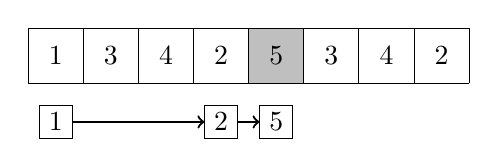
\begin{tikzpicture}[scale=0.7]
\fill[color=lightgray] (4,0) rectangle (5,1);
\draw (0,0) grid (8,1);

\node at (0.5,0.5) {$1$};
\node at (1.5,0.5) {$3$};
\node at (2.5,0.5) {$4$};
\node at (3.5,0.5) {$2$};
\node at (4.5,0.5) {$5$};
\node at (5.5,0.5) {$3$};
\node at (6.5,0.5) {$4$};
\node at (7.5,0.5) {$2$};

\draw (0.2,0.2-1.2) rectangle (0.8,0.8-1.2);
\draw (3.2,0.2-1.2) rectangle (3.8,0.8-1.2);
\draw (4.2,0.2-1.2) rectangle (4.8,0.8-1.2);

\node at (0.5,0.5-1.2) {$1$};
\node at (3.5,0.5-1.2) {$2$};
\node at (4.5,0.5-1.2) {$5$};

\draw[->,thick] (0.8,0.5-1.2) -- (3.2,0.5-1.2);
\draw[->,thick] (3.8,0.5-1.2) -- (4.2,0.5-1.2);
\end{tikzpicture}
\end{center}

Nakon toga element 5 uklanja se sa stoga
i elementi 3 i 4 dodaju se na stog:
\begin{center}
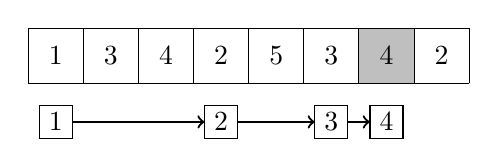
\begin{tikzpicture}[scale=0.7]
\fill[color=lightgray] (6,0) rectangle (7,1);
\draw (0,0) grid (8,1);

\node at (0.5,0.5) {$1$};
\node at (1.5,0.5) {$3$};
\node at (2.5,0.5) {$4$};
\node at (3.5,0.5) {$2$};
\node at (4.5,0.5) {$5$};
\node at (5.5,0.5) {$3$};
\node at (6.5,0.5) {$4$};
\node at (7.5,0.5) {$2$};

\draw (0.2,0.2-1.2) rectangle (0.8,0.8-1.2);
\draw (3.2,0.2-1.2) rectangle (3.8,0.8-1.2);
\draw (5.2,0.2-1.2) rectangle (5.8,0.8-1.2);
\draw (6.2,0.2-1.2) rectangle (6.8,0.8-1.2);

\node at (0.5,0.5-1.2) {$1$};
\node at (3.5,0.5-1.2) {$2$};
\node at (5.5,0.5-1.2) {$3$};
\node at (6.5,0.5-1.2) {$4$};

\draw[->,thick] (0.8,0.5-1.2) -- (3.2,0.5-1.2);
\draw[->,thick] (3.8,0.5-1.2) -- (5.2,0.5-1.2);
\draw[->,thick] (5.8,0.5-1.2) -- (6.2,0.5-1.2);
\end{tikzpicture}
\end{center}

Na kraju se svi elementi osim 1 uklanjaju
sa stoga, a posljednji element 2
dodaje se na stog:

\begin{center}
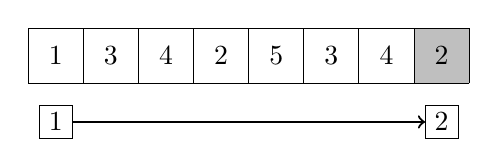
\begin{tikzpicture}[scale=0.7]
\fill[color=lightgray] (7,0) rectangle (8,1);
\draw (0,0) grid (8,1);

\node at (0.5,0.5) {$1$};
\node at (1.5,0.5) {$3$};
\node at (2.5,0.5) {$4$};
\node at (3.5,0.5) {$2$};
\node at (4.5,0.5) {$5$};
\node at (5.5,0.5) {$3$};
\node at (6.5,0.5) {$4$};
\node at (7.5,0.5) {$2$};

\draw (0.2,0.2-1.2) rectangle (0.8,0.8-1.2);
\draw (7.2,0.2-1.2) rectangle (7.8,0.8-1.2);

\node at (0.5,0.5-1.2) {$1$};
\node at (7.5,0.5-1.2) {$2$};

\draw[->,thick] (0.8,0.5-1.2) -- (7.2,0.5-1.2);
\end{tikzpicture}
\end{center}

Efikasnost algoritma ovisi o
ukupnom broju operacija nad stogom.
Ako je trenutni element veći od
elementa na vrhu stoga, izravno se
dodaje na stog, što je efikasno.
Ipak, ponekad stog može sadržavati nekoliko
većih elemenata i potrebno je vrijeme da ih se ukloni.
No svaki element dodaje se \emph{točno jednom} na stog
i uklanja \emph{najviše jednom} sa stoga.
Dakle, svaki element uzrokuje $O(1)$ operacija nad stogom,
i algoritam radi u $O(n)$ vremenu.

\section{Minimum pomičnog prozora}

\index{pomični prozor}
\index{minimum pomičnog prozora}

\key{Pomični prozor} je podniz konstantne veličine
koji se kreće slijeva nadesno kroz niz.
Na svakom položaju prozora
želimo izračunati neku informaciju
o elementima unutar prozora.
U ovom odjeljku usredotočujemo se na zadatak
održavanja \key{minimuma pomičnog prozora},
što znači da
trebamo javiti najmanju vrijednost unutar svakog prozora.

Minimum pomičnog prozora može se izračunati
koristeći sličnu ideju kao onu kojom smo računali
najbliže manje elemente.
Održavamo red
u kojem je svaki element veći od
prethodnog elementa,
a prvi element
uvijek odgovara najmanjem elementu unutar prozora.
Nakon svakog pomaka prozora
uklanjamo elemente s kraja reda
dok posljednji element reda
ne postane manji od novog elementa prozora,
ili dok red ne ostane prazan.
Također uklanjamo prvi element reda
ako više nije unutar prozora.
Na kraju dodajemo novi element prozora
na kraj reda.

Kao primjer, razmotrimo sljedeći niz:

\begin{center}
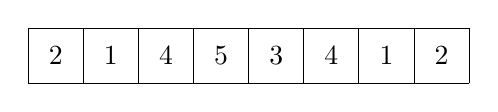
\begin{tikzpicture}[scale=0.7]
\draw (0,0) grid (8,1);

\node at (0.5,0.5) {$2$};
\node at (1.5,0.5) {$1$};
\node at (2.5,0.5) {$4$};
\node at (3.5,0.5) {$5$};
\node at (4.5,0.5) {$3$};
\node at (5.5,0.5) {$4$};
\node at (6.5,0.5) {$1$};
\node at (7.5,0.5) {$2$};
\end{tikzpicture}
\end{center}

Pretpostavimo da je veličina pomičnog prozora 4.
Na prvom položaju prozora najmanja vrijednost je 1:
\begin{center}
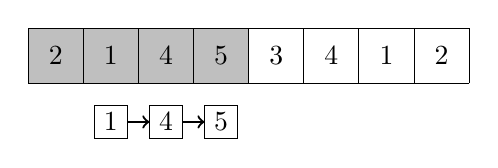
\begin{tikzpicture}[scale=0.7]
\fill[color=lightgray] (0,0) rectangle (4,1);
\draw (0,0) grid (8,1);

\node at (0.5,0.5) {$2$};
\node at (1.5,0.5) {$1$};
\node at (2.5,0.5) {$4$};
\node at (3.5,0.5) {$5$};
\node at (4.5,0.5) {$3$};
\node at (5.5,0.5) {$4$};
\node at (6.5,0.5) {$1$};
\node at (7.5,0.5) {$2$};

\draw (1.2,0.2-1.2) rectangle (1.8,0.8-1.2);
\draw (2.2,0.2-1.2) rectangle (2.8,0.8-1.2);
\draw (3.2,0.2-1.2) rectangle (3.8,0.8-1.2);

\node at (1.5,0.5-1.2) {$1$};
\node at (2.5,0.5-1.2) {$4$};
\node at (3.5,0.5-1.2) {$5$};

\draw[->,thick] (1.8,0.5-1.2) -- (2.2,0.5-1.2);
\draw[->,thick] (2.8,0.5-1.2) -- (3.2,0.5-1.2);
\end{tikzpicture}
\end{center}

Zatim se prozor pomiče jedan korak udesno.
Novi element 3 manji je od elemenata
4 i 5 u redu, pa se elementi 4 i 5
uklanjaju iz reda,
a element 3 dodaje se u red.
Najmanja vrijednost još je uvijek 1.
\begin{center}
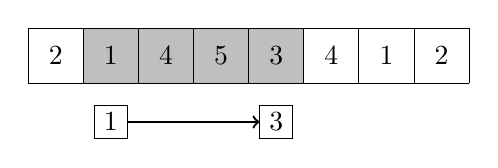
\begin{tikzpicture}[scale=0.7]
\fill[color=lightgray] (1,0) rectangle (5,1);
\draw (0,0) grid (8,1);

\node at (0.5,0.5) {$2$};
\node at (1.5,0.5) {$1$};
\node at (2.5,0.5) {$4$};
\node at (3.5,0.5) {$5$};
\node at (4.5,0.5) {$3$};
\node at (5.5,0.5) {$4$};
\node at (6.5,0.5) {$1$};
\node at (7.5,0.5) {$2$};

\draw (1.2,0.2-1.2) rectangle (1.8,0.8-1.2);
\draw (4.2,0.2-1.2) rectangle (4.8,0.8-1.2);

\node at (1.5,0.5-1.2) {$1$};
\node at (4.5,0.5-1.2) {$3$};

\draw[->,thick] (1.8,0.5-1.2) -- (4.2,0.5-1.2);
\end{tikzpicture}
\end{center}

Nakon toga prozor se ponovno pomiče,
i najmanji element 1
više ne pripada prozoru.
Dakle, uklanja se iz reda i najmanja
vrijednost sada je 3. Također se novi element 4
dodaje u red.
\begin{center}
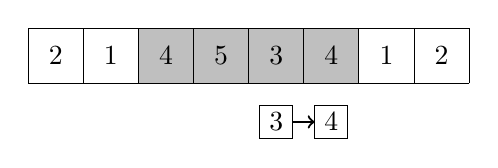
\begin{tikzpicture}[scale=0.7]
\fill[color=lightgray] (2,0) rectangle (6,1);
\draw (0,0) grid (8,1);

\node at (0.5,0.5) {$2$};
\node at (1.5,0.5) {$1$};
\node at (2.5,0.5) {$4$};
\node at (3.5,0.5) {$5$};
\node at (4.5,0.5) {$3$};
\node at (5.5,0.5) {$4$};
\node at (6.5,0.5) {$1$};
\node at (7.5,0.5) {$2$};

\draw (4.2,0.2-1.2) rectangle (4.8,0.8-1.2);
\draw (5.2,0.2-1.2) rectangle (5.8,0.8-1.2);

\node at (4.5,0.5-1.2) {$3$};
\node at (5.5,0.5-1.2) {$4$};

\draw[->,thick] (4.8,0.5-1.2) -- (5.2,0.5-1.2);
\end{tikzpicture}
\end{center}

Sljedeći novi element 1 manji je od svih elemenata
u redu.
Dakle, svi elementi uklanjaju se iz reda
i on će sadržavati samo element 1:
\begin{center}
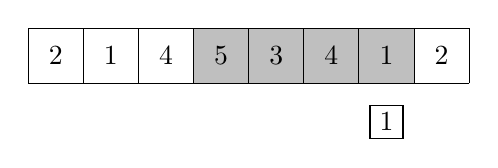
\begin{tikzpicture}[scale=0.7]
\fill[color=lightgray] (3,0) rectangle (7,1);
\draw (0,0) grid (8,1);

\node at (0.5,0.5) {$2$};
\node at (1.5,0.5) {$1$};
\node at (2.5,0.5) {$4$};
\node at (3.5,0.5) {$5$};
\node at (4.5,0.5) {$3$};
\node at (5.5,0.5) {$4$};
\node at (6.5,0.5) {$1$};
\node at (7.5,0.5) {$2$};

\draw (6.2,0.2-1.2) rectangle (6.8,0.8-1.2);

\node at (6.5,0.5-1.2) {$1$};
\end{tikzpicture}
\end{center}

Na kraju prozor dolazi na svoj posljednji položaj.
Element 2 dodaje se u red,
ali najmanja vrijednost unutar prozora
još je uvijek 1.
\begin{center}
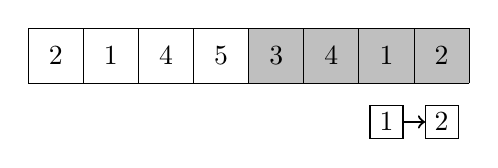
\begin{tikzpicture}[scale=0.7]
\fill[color=lightgray] (4,0) rectangle (8,1);
\draw (0,0) grid (8,1);

\node at (0.5,0.5) {$2$};
\node at (1.5,0.5) {$1$};
\node at (2.5,0.5) {$4$};
\node at (3.5,0.5) {$5$};
\node at (4.5,0.5) {$3$};
\node at (5.5,0.5) {$4$};
\node at (6.5,0.5) {$1$};
\node at (7.5,0.5) {$2$};

\draw (6.2,0.2-1.2) rectangle (6.8,0.8-1.2);
\draw (7.2,0.2-1.2) rectangle (7.8,0.8-1.2);

\node at (6.5,0.5-1.2) {$1$};
\node at (7.5,0.5-1.2) {$2$};

\draw[->,thick] (6.8,0.5-1.2) -- (7.2,0.5-1.2);
\end{tikzpicture}
\end{center}

Budući da se svaki element niza
dodaje u red točno jednom i
uklanja iz reda najviše jednom,
algoritam radi u $O(n)$ vremenu.



